\section{Barrel Silicon Vertex Tracker (BST)}


\subsection{Geometry}


The BST geometry is implemented through the COATJAVA geometry service.
The service provides the Geant4 definitions that are read by the GEMC perl API to build the geometry database.

There are three BST regions, with 10, 14, and 18 sectors/modules for region 1, 2, and 3 respectively, see \F{bstGeometry}.
Each module has six sensors, four readout chips, and several layers of material,
including (length of line represents depth level):

\begin{itemize}
	\item -- wirebond
	\item ---- silicon
	\item ------ epoxy
	\item -------- rail
	\item ---------- bus cable
	\item ------------ carbon fiber
	\item -------------- rohacell
	\item ------------ carbon fiber
	\item ---------- bus cable
	\item -------- rail
	\item ------ epoxy
	\item ---- silicon
	\item -- wirebond
\end{itemize}

The active area of the slilicon sensor is associated with the BST hit process routine.
The strip identification is performed in the Process ID routine.

\begin{figure}
	\centering
	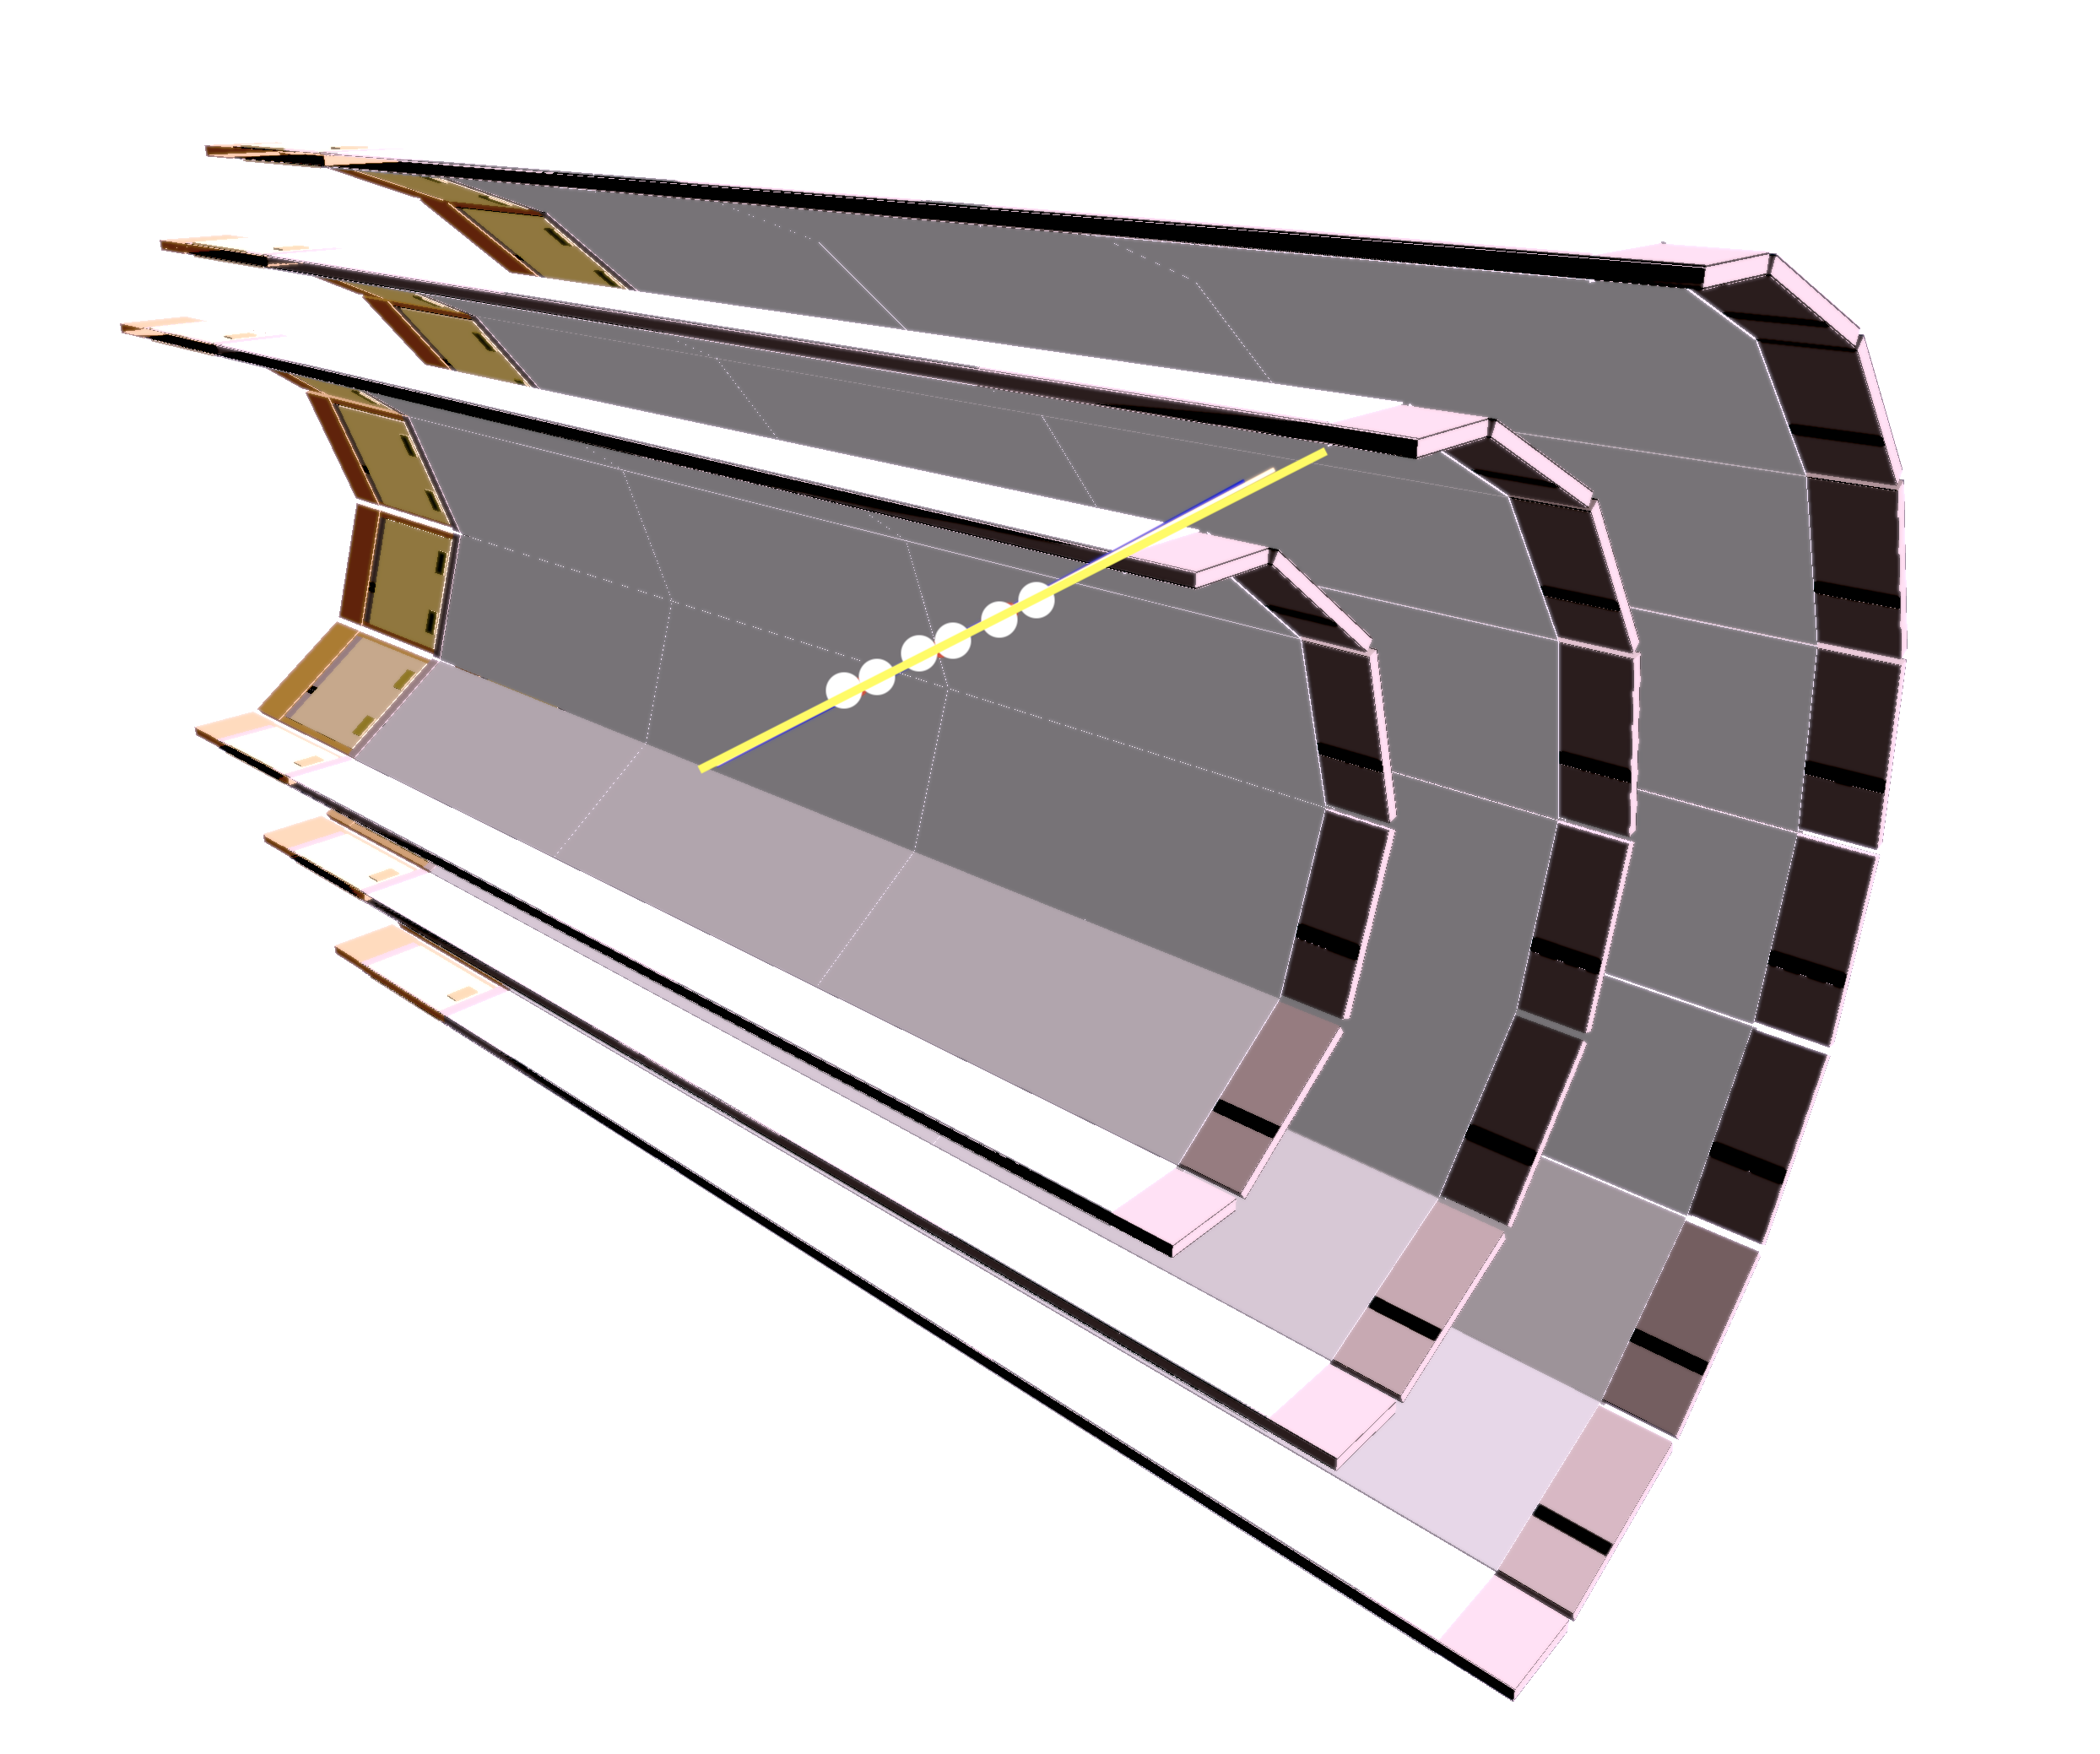
\includegraphics[width=0.95\columnwidth,keepaspectratio]{img/bstGeometry.png}
	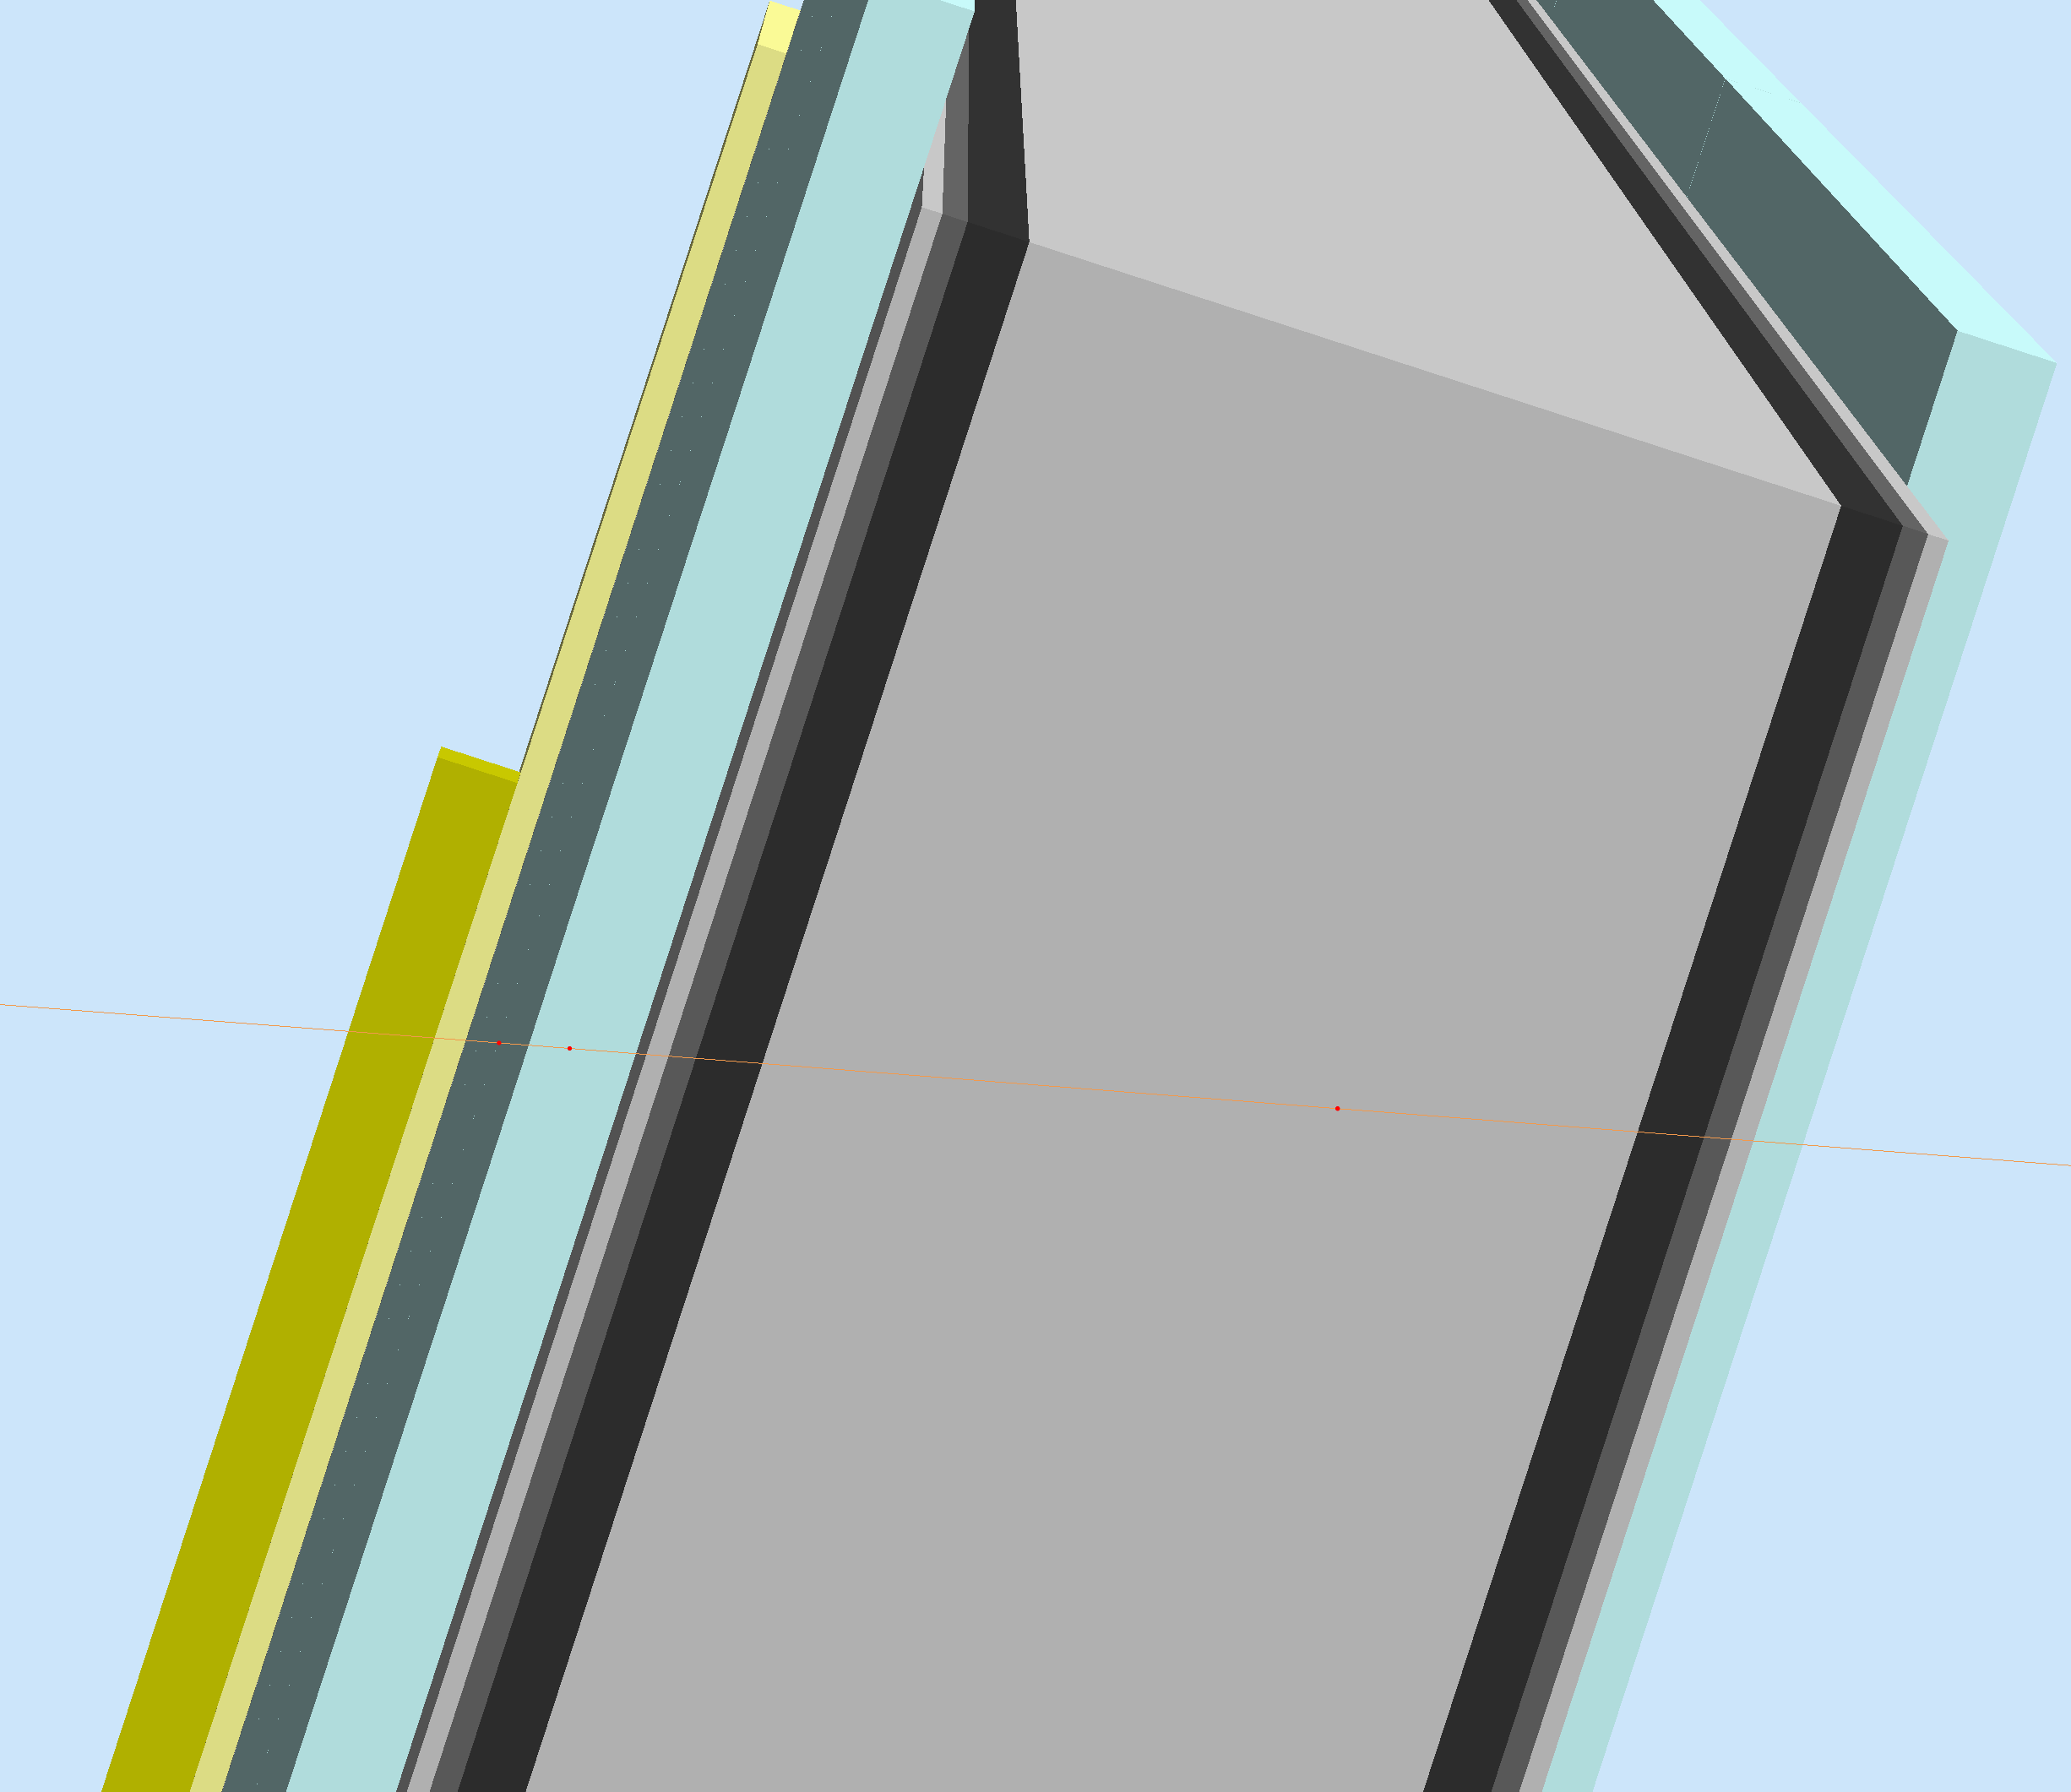
\includegraphics[width=0.95\columnwidth,keepaspectratio]{img/bstDetail.png}
	\caption{Top: the GEMC implementation of the BST geometry. The three regions are shown in the sliced view. The silicon sensors are shown
           in cyan color. The blue track is a 2 GeV proton, leaving hits in each module crossed. Bottom: detail of a module shows
           the various material inside. The 320 $\mu$ m silicon sensor is on top and bottom of the module.
           The material inside includes epoxy glue, the bus cable, and support material. }
	\label{fig:bstGeometry}
\end{figure}


\subsubsection{Geometry Location on GitHub}
The Github location of the GEMC perl API script is at \url{https://github.com/gemc/detectors/tree/master/clas12/bst}.
The geometry service definitions in coatjava is at
\url{https://github.com/JeffersonLab/clas12-offline-software/blob/development/common-tools/clas-jcsg/src/main/java/org/jlab/detector/geant4/v2/SVTGeant4Factory.java}


\subsection{Process ID}

At each Geant4 step, the local coordinates in the sensor volume are used to calculate the strip id.
The algorithm includes: the dead zone around the sensor, the pitch between the strips (156 $\mu$ m) and the angle
between the strips, that varies from 0 (strip n. 1) to 3 degrees (for strip n. 256). A showcase of the strip id assignment
is summarized in \F{processID}.

\begin{figure}
	\centering
	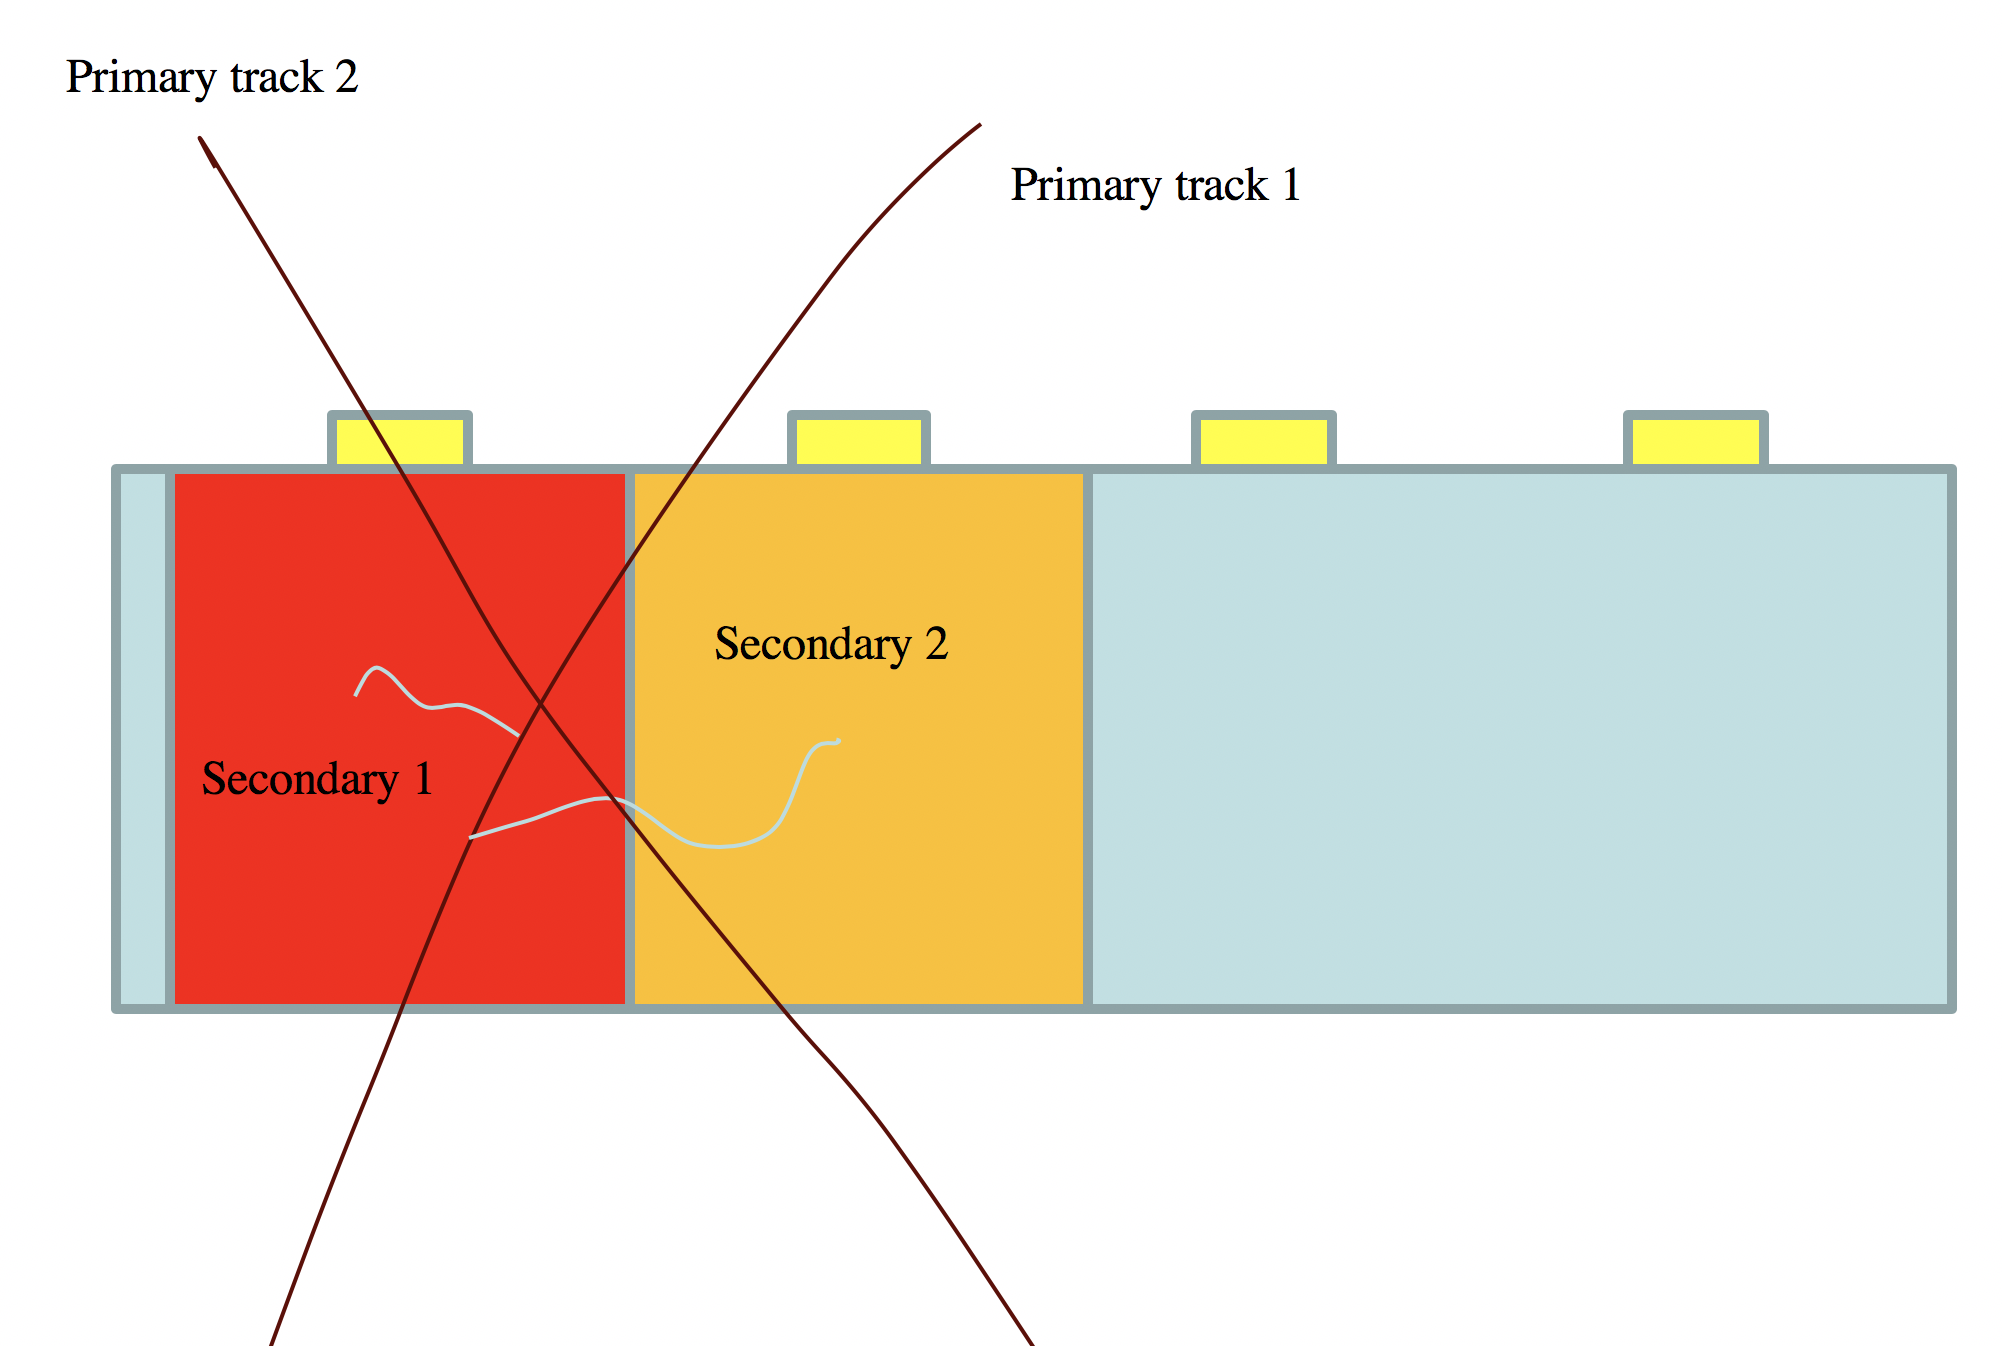
\includegraphics[width=0.95\columnwidth,keepaspectratio]{img/bstHit.png}
	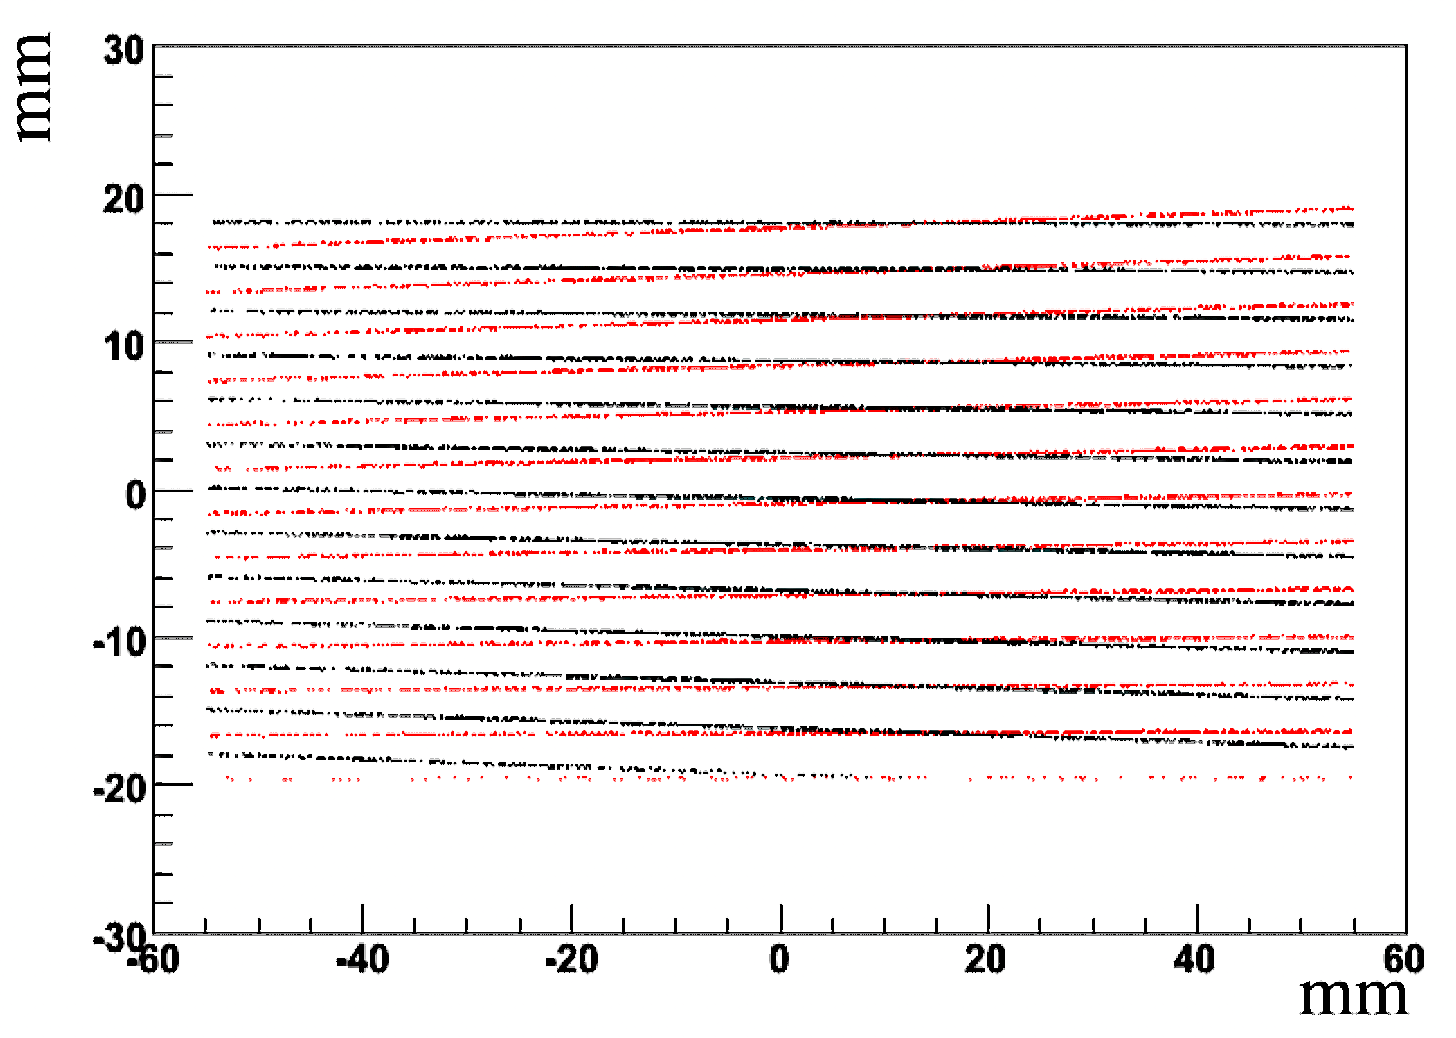
\includegraphics[width=0.95\columnwidth,keepaspectratio]{img/bstStrip.png}
	\caption{Top: process ID algorithm cartoon for BST. The strip ID is assigned based on the local position of the track
            step within the sensitive module. If a step of the primary or the secondary particles happen between the boundary
            of the strip that was already hit, it will be assigned to that strip. Bottom: actual hit position of selected
            strips in the top and bottom silicon sensors of a module shows the fan-like distribution of the strips,
            with increasing angle. The top layer angle is opposite to the bottom layer angle. }
	\label{fig:processID}
\end{figure}

Due to the thickness of the silicon sensor, the electrons avalanche produced can end up in more than one strip. This
is reproduced in the GEMC simulation using the hit sharing algorithm, see \F{bstHitSharing}.

\begin{figure}[t]
	\centering
	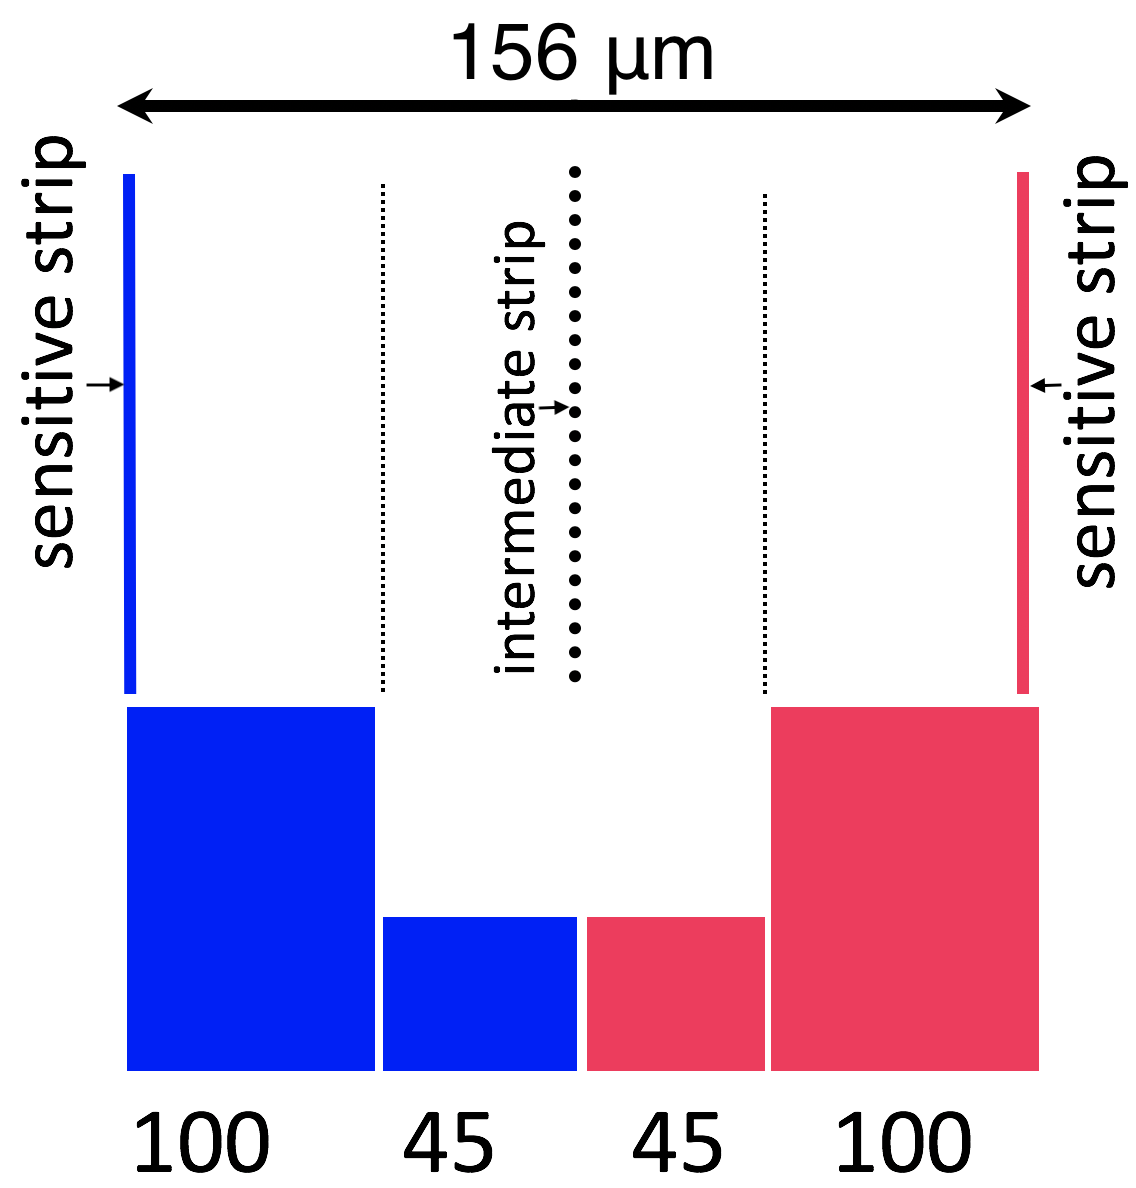
\includegraphics[width=0.95\columnwidth,keepaspectratio]{img/bstHitSharing.png}
	\caption{The BST hit sharing algorithm. If a step in a given strip happens from within 39 $\mu$ m the adjacent strip, then
            $90\%$ of the energy deposited will be shared equally between them ($45\%$ each), with a $10\%$ energy loss due
	         to capacitive coupling between the strip and the backplane.}
	\label{fig:bstHitSharing}
\end{figure}


\subsection{Digitization}

\subsubsection{ADC}
The BST digitization provides a 3 bit ADC, using the total energy deposited (after hit sharing) between 26 and 117 keV.

\subsubsection{TDC}
The Bunch Cross Oscillator quantity (BCO), a random number between 0 and 255,
provides the timing info associated with the hit.

\subsection{Digitized Bank}
The digitized output bank has $ID=100$, and the variables are summarized in Table \ref{tab:bstBank}.

\begin{table}[h]
	\begin{center}
		\begin{tabular}{| c | c | c |}
			\hline \hline
			Variable         & Description  & Tag  \\
			\hline
               layer  &                                      layer number  &    1   \\
              sector  &                                     sector number  &    2   \\
               strip  &                                      strip number  &    3   \\
                 ADC  &                                         3 bit ADC  &    4   \\
                 bco  &                                   8 bit time info  &    5   \\
               ADCHD  &                                        13 bit ADC  &    6   \\
                time  &                                  Time information  &    7   \\
                hitn  &                                        hit number  &   99   \\
			\hline \hline
		\end{tabular}
	\end{center}
	\caption{The digitized BST bank.}\label{tab:bstBank}
\end{table}


\subsubsection{Time Window}
The time window  of the BST is set to to 128 ns.

\subsubsection{Process Routine Git Repository Location}

The BST hit process routines are located in the repository: \url{https://github.com/gemc/source/tree/master/hitprocess/clas12/svt}

\subsubsection{Radiation dose and background rates}
A detailed study of the background rates coming from beam interacting with the target was done to ensure that the silicon sensor
could operate in the high radiation conditions of the target proximity.

Given the nominal operating luminosity $L=10^{35} cm^{-2}s^{-1}$, and the liquid-Hydrogen target of 5 cm thickness, the beam electron rate
is $R=4.7 \times 10^{11} Hz$. This corresponds to about 62,000 electrons in the BST 128 ns time window.

Simulations using 62,000 11 GeV electrons per event impinging on the liquid-Hydrogen target were analyzed.

The rates were calculated for the various regions and for different thresholds.
The radiation dose and the 1 MeV neutron equivalent damage was estimated. Most of the radiation
is released in the first two layers of the BST.
The 370 rad / year are low enough to grant the BST operation for 15 years. The results of the study
are summarized in \F{radStudy}.

In addition a thin layer of tungsten was added between the target and the inner BST layer aimed at reducing the electromagnetic
background \cite{bstDose}.

\begin{figure}
	\centering
	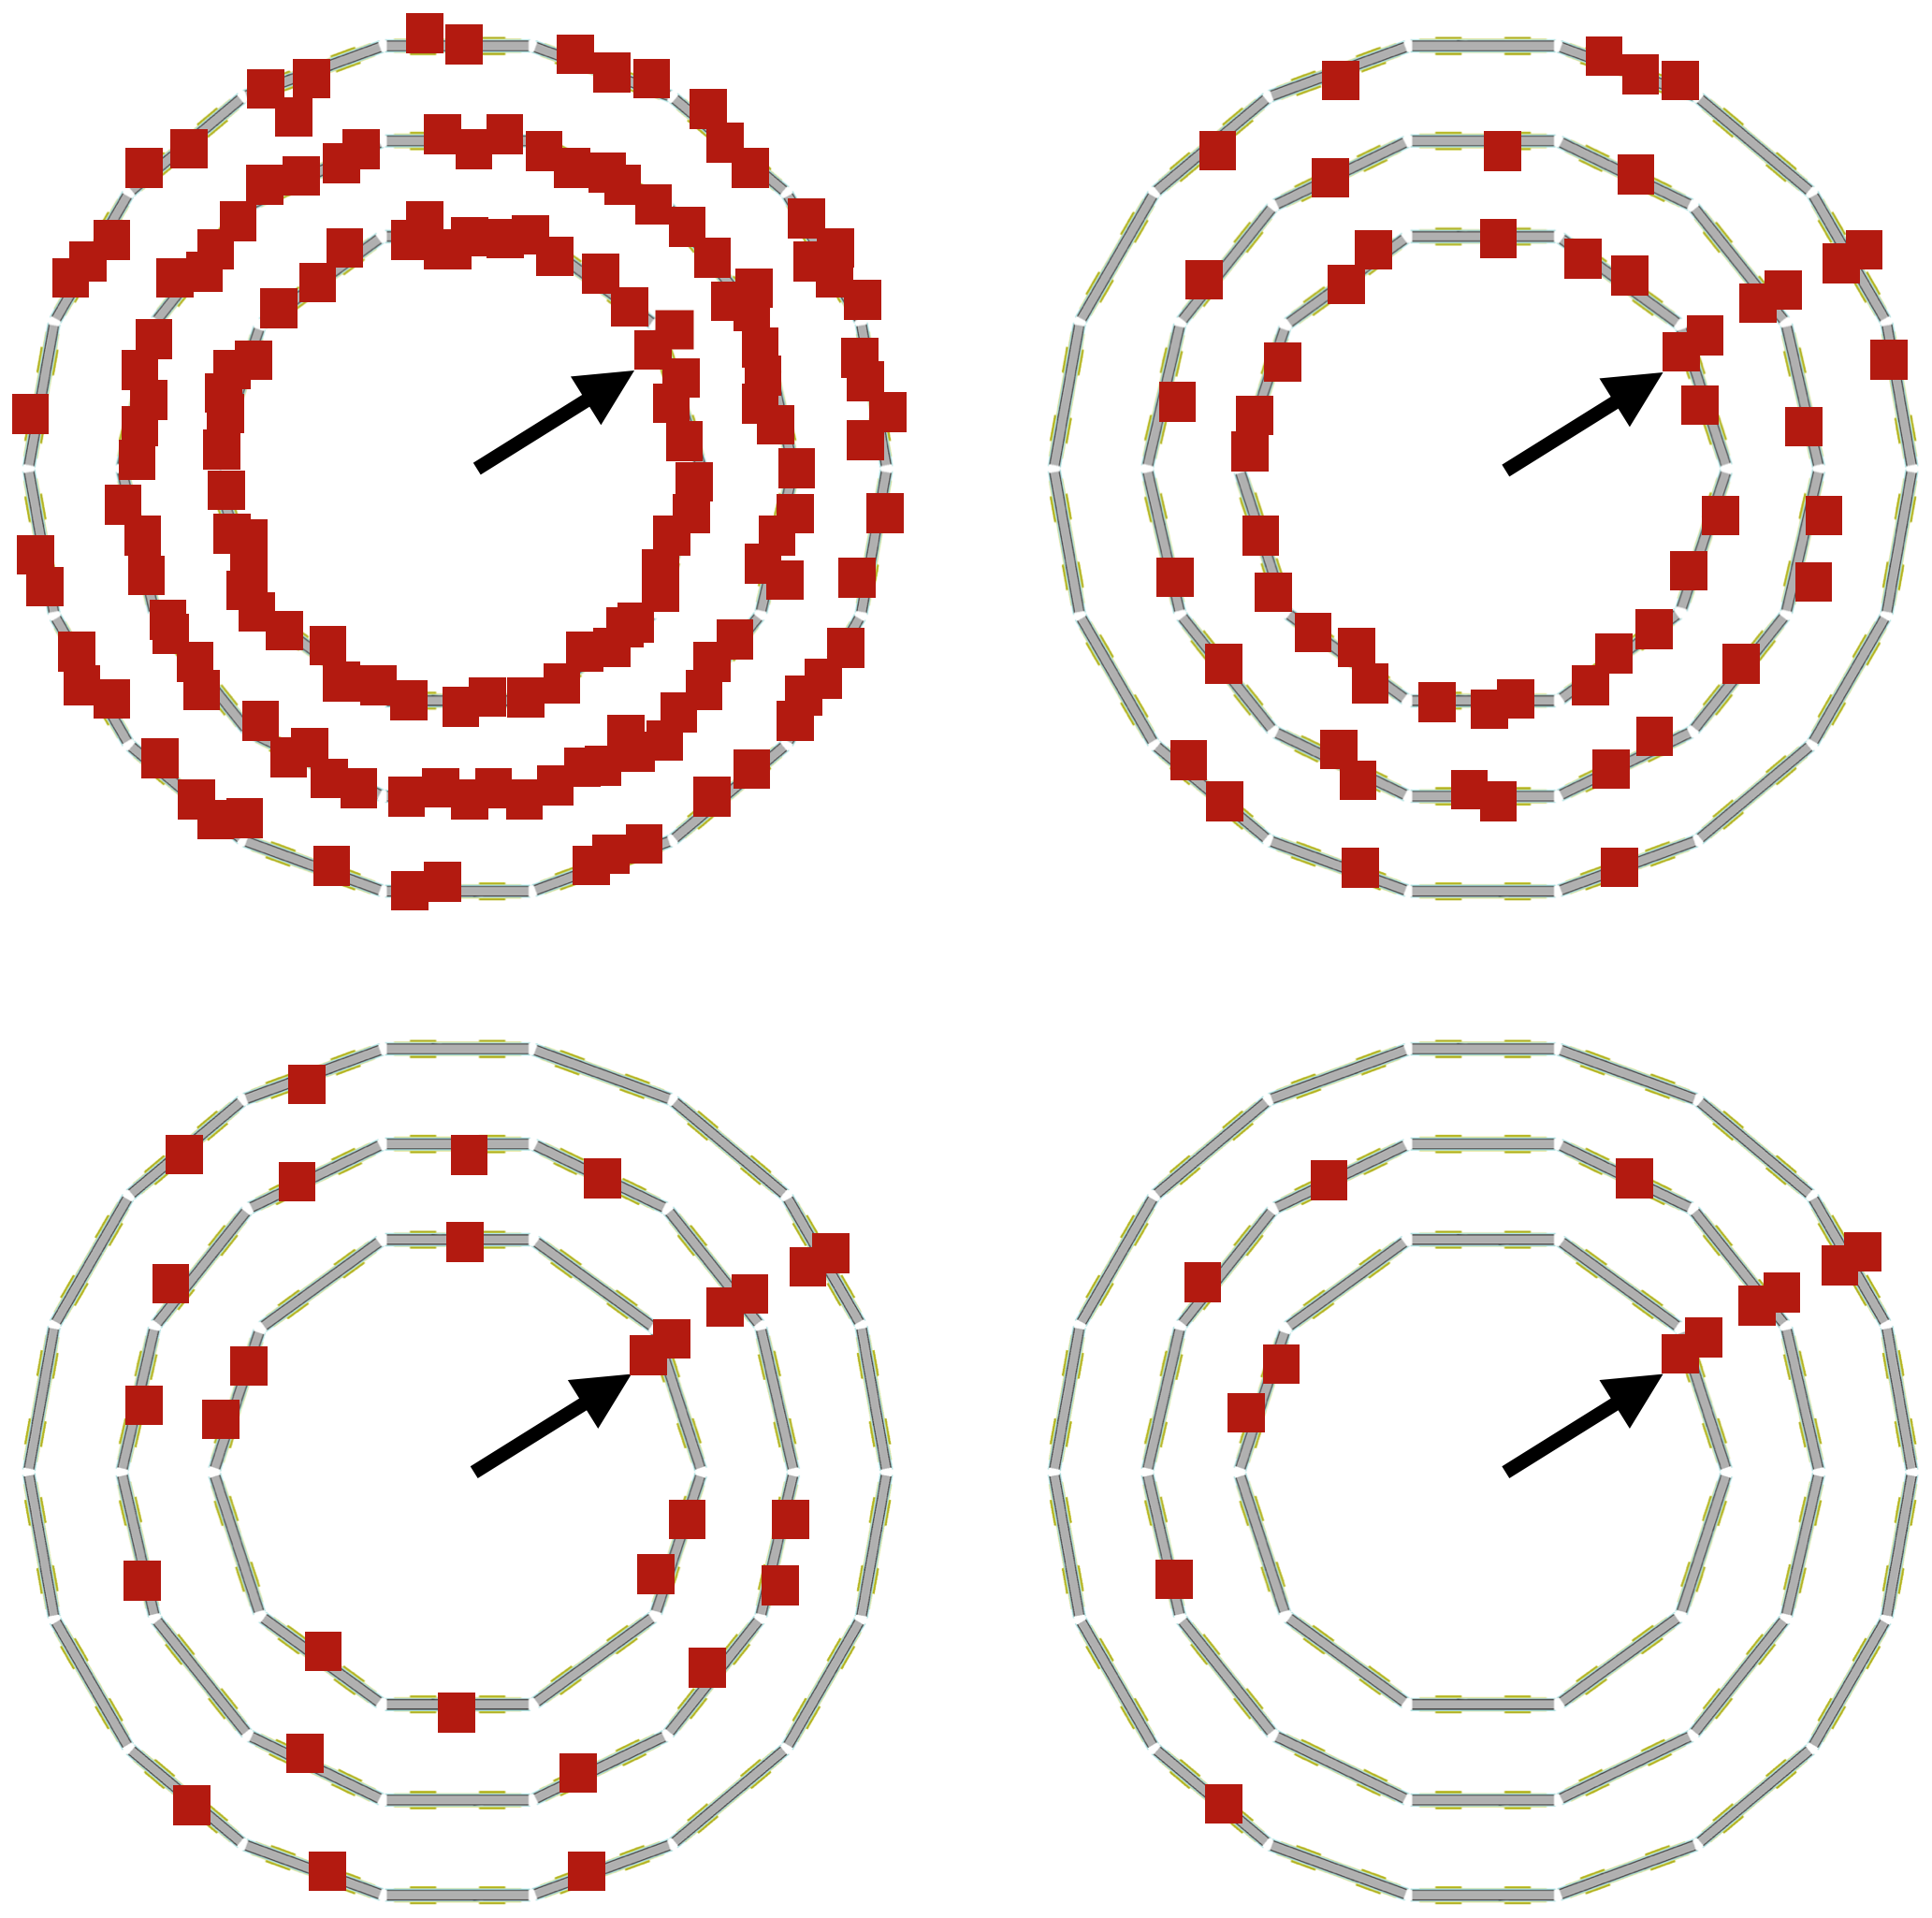
\includegraphics[width=0.95\columnwidth,keepaspectratio]{img/bstHitDisplay.png}
	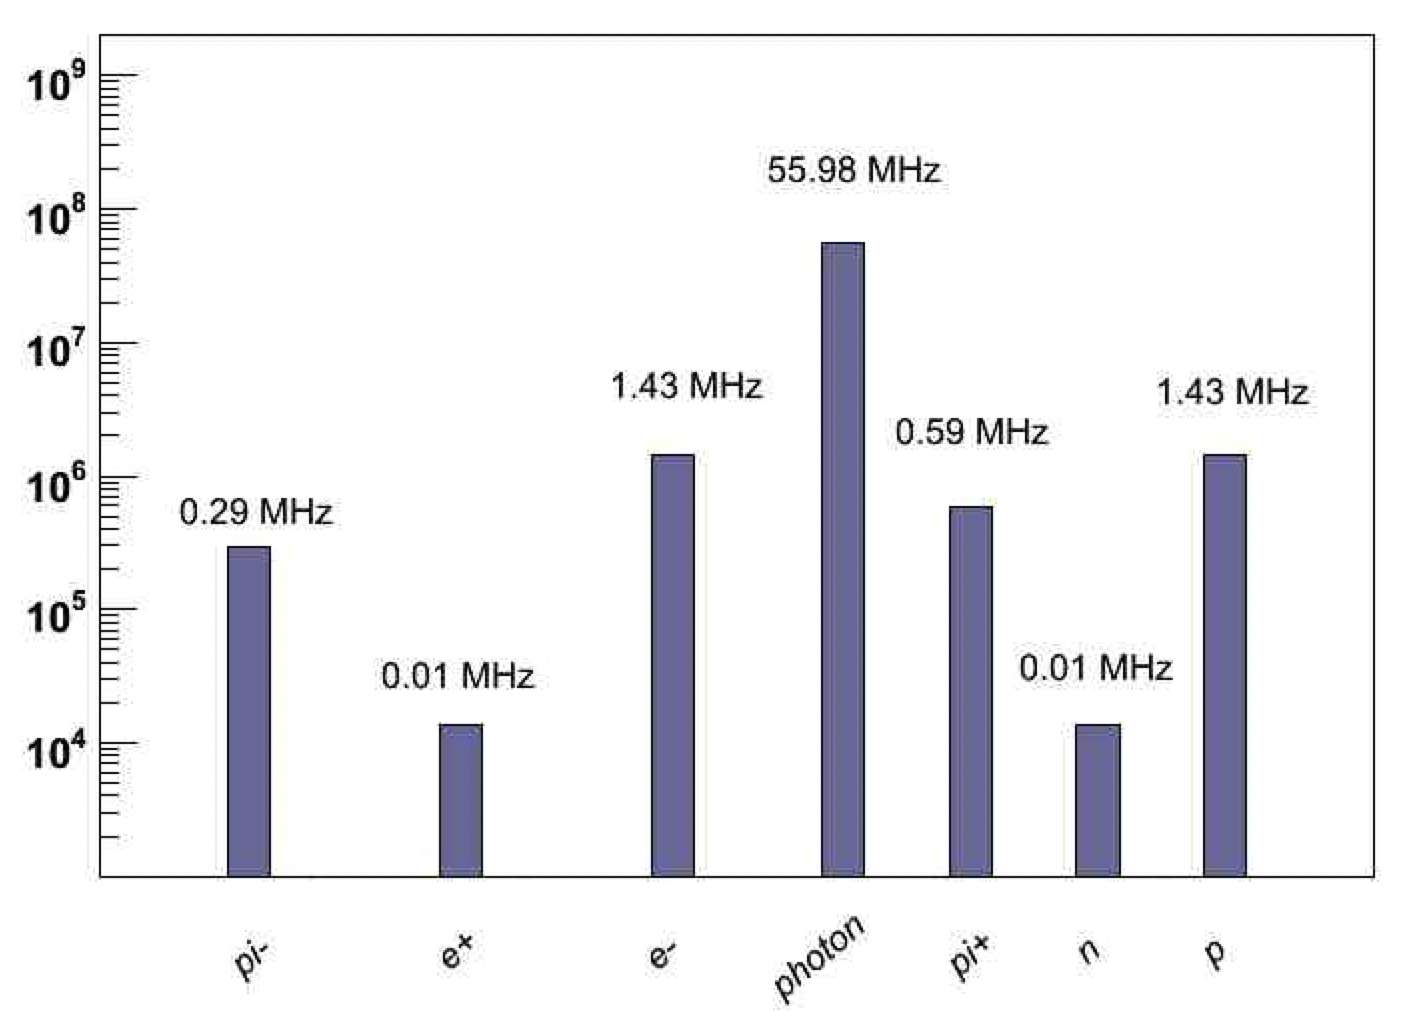
\includegraphics[width=0.95\columnwidth,keepaspectratio]{img/bstRates.png}
	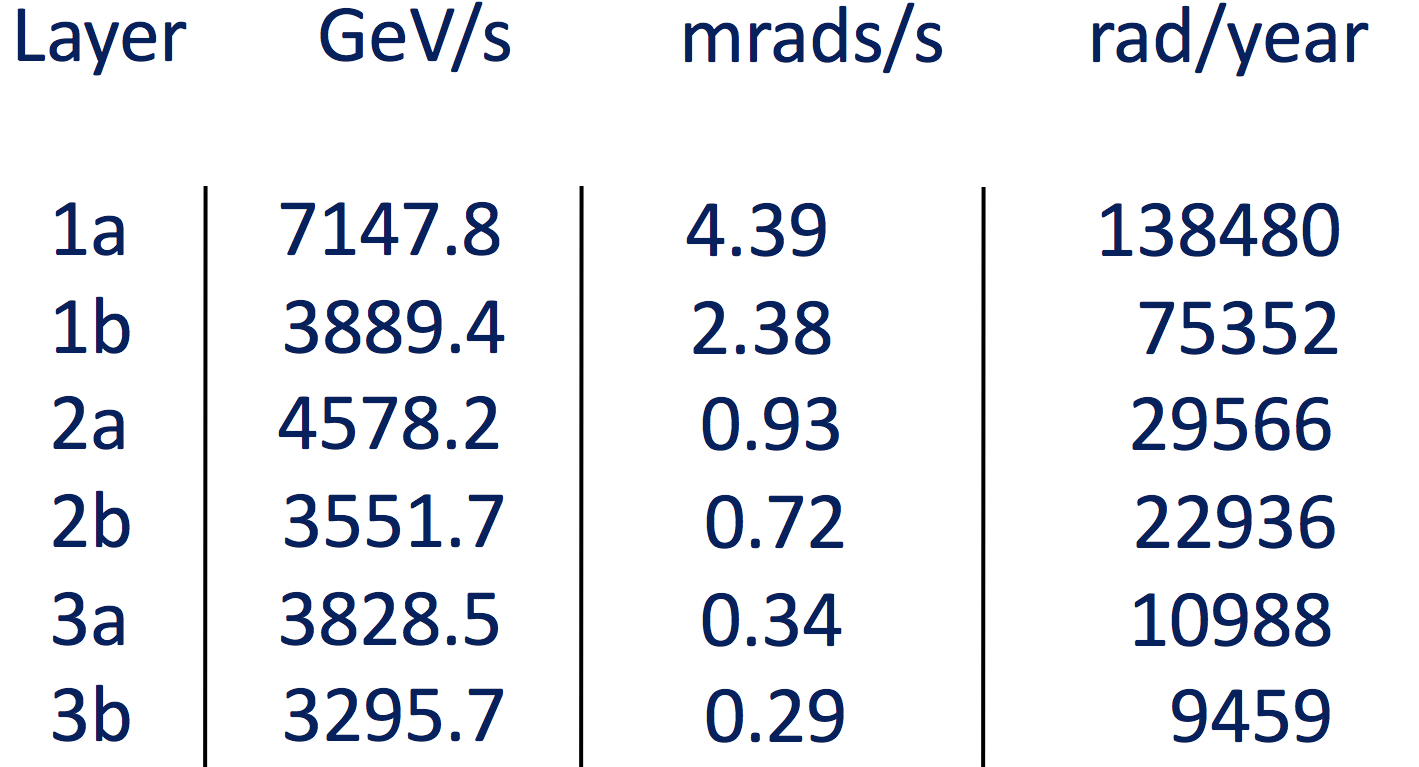
\includegraphics[width=0.95\columnwidth,keepaspectratio]{img/bstRadSummary.png}
	\caption{Summary of radiation doses and background rates in the BST. Top: the occupancy in the various BST layers
            for different thresholds. Middle: the rate breakdown for different particles for a threshold of 20 keV.
            The current hardware threshold is 30 keV. Bottom: table showing the fluences and radiation doses in the BST
            layers. }
	\label{fig:radStudy}
\end{figure}



